\documentclass[a4paper]{article}

\usepackage{amsthm}
\usepackage{amsmath}
\usepackage{amssymb}
\usepackage{multirow}
\usepackage{graphicx}
\usepackage[margin=2.5cm]{geometry}
\usepackage{hyperref}
\usepackage{color}
\usepackage{titlesec}
\PassOptionsToPackage{obeyspaces}{url}
\usepackage{url}
\usepackage{graphicx}
\usepackage{wrapfig}
\usepackage{multicol}

\titlespacing\subsubsection{0pt}{2pt plus 4pt minus 2pt}{2pt plus 2pt minus 2pt}

\newcommand{\code}{\texttt}

\title{\vspace{-5ex}Trivial File Transfer Protocol}
\author{153728}
\date{}

\begin{document}
\maketitle
\vspace{-4ex}

\begin{center}
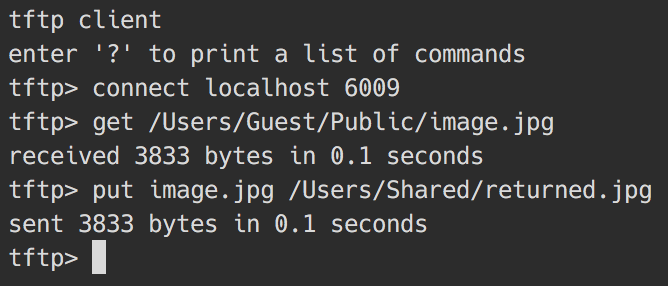
\includegraphics[width=0.5\textwidth]{image}
\end{center}

\section{Core}

In implementing the Trivial File Transfer Protocol, I attempted to abstract as much as possible so that a large amount of code could be shared between the client and server applications (in both the UDP version and the TCP version). So initially, I focused on translating the specifications of the TFTP to `Java representation'. The \code{tftp.core} package contains enums describing error types (e.g. \code{ErrorType.FILE\_NOT\_FOUND}), transfer modes (e.g. \code{Mode.OCTET}) and classes describing TFTP packets (e.g. \code{WriteRequestPacket} and \code{DataPacket}). Each of these TFTP packet classes inherit from a base class \code{TFTPPacket}. Each TFTPPacket subclass has two constructors - one for creating a new TFTPPacket from `logical data' (e.g. \code{new ErrorPacket(ErrorType.FILE\_NOT\_FOUND, "file")}), and another for parsing the packet from a byte buffer. Byte array parsing is done using a \code{ByteBuffer} wrapping the buffer. The parent class \code{TFTPPacket} contains a static method \code{fromByteArray} which takes a byte buffer (and length) and returns a \code{TFTPPacket}. This was done by examining the first two bytes (the opcode) of the packet and then, based on this opcode, instantiating the relevant \code{TFTPPacket} subclass.

\section{UDP TFTP}

\subsection{Server}

The \code{TFTPUDPServer} program takes two optional arguments: \code{-port port-number} to set the port to bind to and \code{-timeout time-in-ms} to set the timeout length - for example,
\begin{center}
\code{java tftp.udp.server.TFTPUDPServer -port 7000 -timeout 4000}.
\end{center}
By default, the server binds to port 6009 and has a timeout of 3000ms.

The main server class \code{TFTPUDPServer} handles accepting write/read requests from clients, and spawning the relevant `worker' thread to send or receive the client-specified file. This is done by binding a datagram socket to a given port (passed to the class constructor), port 6009 in my implementation. From there, a buffer to hold received packets is allocated, and then the server infinitely loops. In each pass through the loop, the socket waits to receive a datagram (blocking). When a datagram is received, the \code{TFTPPacket} is extracted from the buffer. Based on the type of request (\code{RRQ} or \code{WRQ}), the server submits a job to an asynchronous \code{ExecutorService} to respond to the request, and the loop repeats.

The two worker classes to respond to read and write requests are \code{ServerWriter} and \code{ServerReader} respectively. Constructors for both these classes accept a client address and client port (to know where to send datagrams), and the original request packet (to obtain the file name and to ensure the transfer is taking place using octet mode).

Upon running, the \code{ServerWriter} creates a new datagram socket and binds it to a random free port. A timeout is also specified based on the server configuration. Then the transfer mode of the RRQ packet is checked - if not \code{Mode.OCTET} then an error packet is sent to the client and the server worker terminates. If the mode is octet however, an input stream is opened to the file specified by the client (if the file does not exist, an error packet is sent to the client and the transfer terminates).

The \code{ServerReader} works similarly.

\subsection{Client}

After writing the server, the client was fairly straightforward because all code for transferring and receiving a file over TFTP had already been done. So most of the work developing the client involved coding the command line interface. My client is modelled after the OS X \code{tftp} program, a TFTP client bundled with OS X. As with the OS X program, entering `?' lists the available commands:
\begin{itemize}
\item \code{connect hostname [port]} sets the hostname/IP address of the TFTP server, and optionally the port. If no port is specified this will use the default port in this TFTP implementation, 6009. This is not connection in the TCP sense, but rather just sets the destination of outgoing datagrams.
\item \code{get remote-path [local-path]} retrieves a file from the connected TFTP server. \code{remote-path} is the path to the file on the server, and \code{local-path} is the path to the file on the local machine. If \code{local-path} is not specified it the file is saved to the working directory. 
\item \code{put local-path [remote-path]} writes a file to the connected TFTP server. \code{local-path} is the path to the file on the local machine, and \code{remote-path} is where the file will be saved on the server - if not specified, it will be in the server's working directory.
\item \code{timeout time-in-ms} sets the timeout length in milliseconds.
\item \code{exit} quits the client.
\end{itemize}

\section{TCP TFTP}

Since TCP provides a reliable transport service for the application layer, the explicit ACKs, timeout handling, etc. are not required in this case. Rather, the protocol can simply involve connecting the receiving a RRQ/WRQ, and then, upon `acceptance' of the request, a direct sending of the file bytes to/from the server. 

\begin{tabular}{ p{0.4\textwidth} p{0.4\textwidth} }
The read request interaction:
\begin{enumerate}
\item client opens connection to server
\item client sends RRQ to server
\item server sends TFTP ACK to indicate that the file transfer has been approved
\item server sends file bytes to client
\item after file is fully sent, server closes connection 
\end{enumerate}
&
The write request interaction:
\begin{enumerate}
\item client opens connection to server
\item client sends WRQ to server
\item server sends TFTP ACK to client (block number is irrelevant, this is just for the server to explicitly approve the transfer)
\item client sends file bytes to server
\item after file is fully sent, client closes connection
\end{enumerate}
\\
\end{tabular}

If the file does not exist, in step 3 the server will send back an error packet instead, containing an error message.

\subsection{Server}

The server first opens a \code{ServerSocket} port on a particular port - by default 6009. The server then blocks until a client connects. When a client connects, a job is submitted to an \code{Executor} to be executed asynchronously - this job is in charge of responding to the client request. The first read from the socket input stream is interpreted as a request packet. The transfer mode of the request packet is ensured to be \code{octet}.

If the packet is a WRQ, the server sends an ACK to the client. Then the file is received by continually reading bytes from the input stream and writing them to file until the connection is closed by the client.

If the packet is a RRQ, the server immediately opens an input stream to the requested file, and sends the file bytes over TCP. Once the sending is complete, the server closes the connection.

\subsection{Client}

The client uses the same structure as the UDP TFTP client, supporting the same commands. The only subtlety is with the \code{connect} command - similarly to the UDP client this does not mean connect in the TCP sense, rather it just sets the server's hostname and port. A separate TCP connection is initiated with every \code{get} and \code{put}.

A \code{get} operation causes a \code{ReadRequestPacket} with the appropriate filename to be sent to the server. Then the client simply receives the file bytes from the server and writes them to file. Once the transfer is complete the server will terminate the TCP connection and the \code{get} operation is complete.

A \code{put} operation causes a \code{WriteRequestPacket} to be sent to the server. The client then waits for an \code{AcknowledgementPacket} to be received from the server. Once received, the client sends the file bytes to the server and closes the connection. 

\end{document}

